%% !TeX root = report.tex

Algorytm IFC (ang. Incremental Frequency Count) został stworzony i przez Jurgena Abela. Algorytm powstał by zaoferować skuteczną metodę przetwarzania danych otrzymanych z BWT. Założeniem było stworzenie algorytmu szybkiego i dającego dobre efekty kompresji. Algorytm został opisany w \cite{abel}. Daje on czasy działania porównywalne z MTF, przy jednoczesnym wysokim stopniu kompresji na poziomie algorytmu Sebastiana Deorowicza - WFC (ang. Weighted Frequency Count)\cite{deorowicz}.  

\begin{figure}
\centering
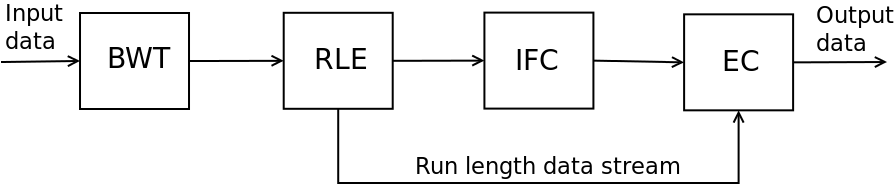
\includegraphics[width=\textwidth]{\PICSDIR/ifc}
\caption{Algorytm kompresji BWT z RLE2 i IFC}
\label{rys:bwca}
\end{figure}

Zadaniem algorytmu drugiej fazy kompresji BWT jest takie przetworzenie struktury z symboli otrzymanych z BWT by była ona łatwa do skompresowania przy użyciu kodeków entropijnych. W celu obliczania wartości wyjściowych w algorytmie IFC każdemu symbolowi przyporządkowywany jest licznik. Wszystkie licznik przechowywane są w kolejności malejącej. Dla każdego odczytanego z wejścia symbolu na wyjście wypisywana jest wartość licznika odpowiadającego temu symbolowi, po czym następuje przeliczenie wartości licznika. Podstawową ideą jest tutaj inkrementacja adaptacyjna bazująca na wykorzystaniu informacji o elementach które już się pojawiły. Liczniki poszczególnych elementów alfabetu mogą być inkrementowane lub dekrementowane w zależności od częstości występowania danego elementu. Powoduje to, że element występujące często mają niższe indeksy. Wartości liczników są co jakiś czas normowane. Główny nacisk kładziony jest w algorytmie na obliczanie wartości inkrementacji liczników. Algorytm podzielony jest na pięć części:
\begin{enumerate}
\item Wypisanie wartości odpowiedniego licznika na wyjście.
\item Obliczenie różnicy dla średniej wartości liczników dla poprzedniego i obecnego znaku. Wartości średnie obliczane są w przesuwnym oknie wg. wzoru:\\
$avg_{i} := \frac{(avg_{i-1} \dot (window\_size - 1)) - index_{x_{i}})}{windows\_size}$
\item Obliczenie wartości inkrementacji na podstawie różnicy średnich i wartości inkrementacji poprzedniego elementu:\\
$inc_i := inc_{i-1} - \frac{inc_{i-1} dif_i}{q}$, gdzie $q$ jest czynnikiem skalującym inkrementacji.
\item Przeskalowanie liczników jeżeli któryś z nich przekroczył wartość graniczną.
\item Ponowne posortowanie liczników. Sprowadza się to do odpowiedniego przesunięcia licznika elementu, który ostatnio pojawił się na wejściu. 
\end{enumerate}